\documentclass{standalone}
\usepackage{tikz}
\usetikzlibrary{patterns, positioning}
\usepackage[sfdefault]{ClearSans} %% option 'sfdefault' activates Clear Sans as the default text font
\usepackage[T1]{fontenc}

\begin{document}
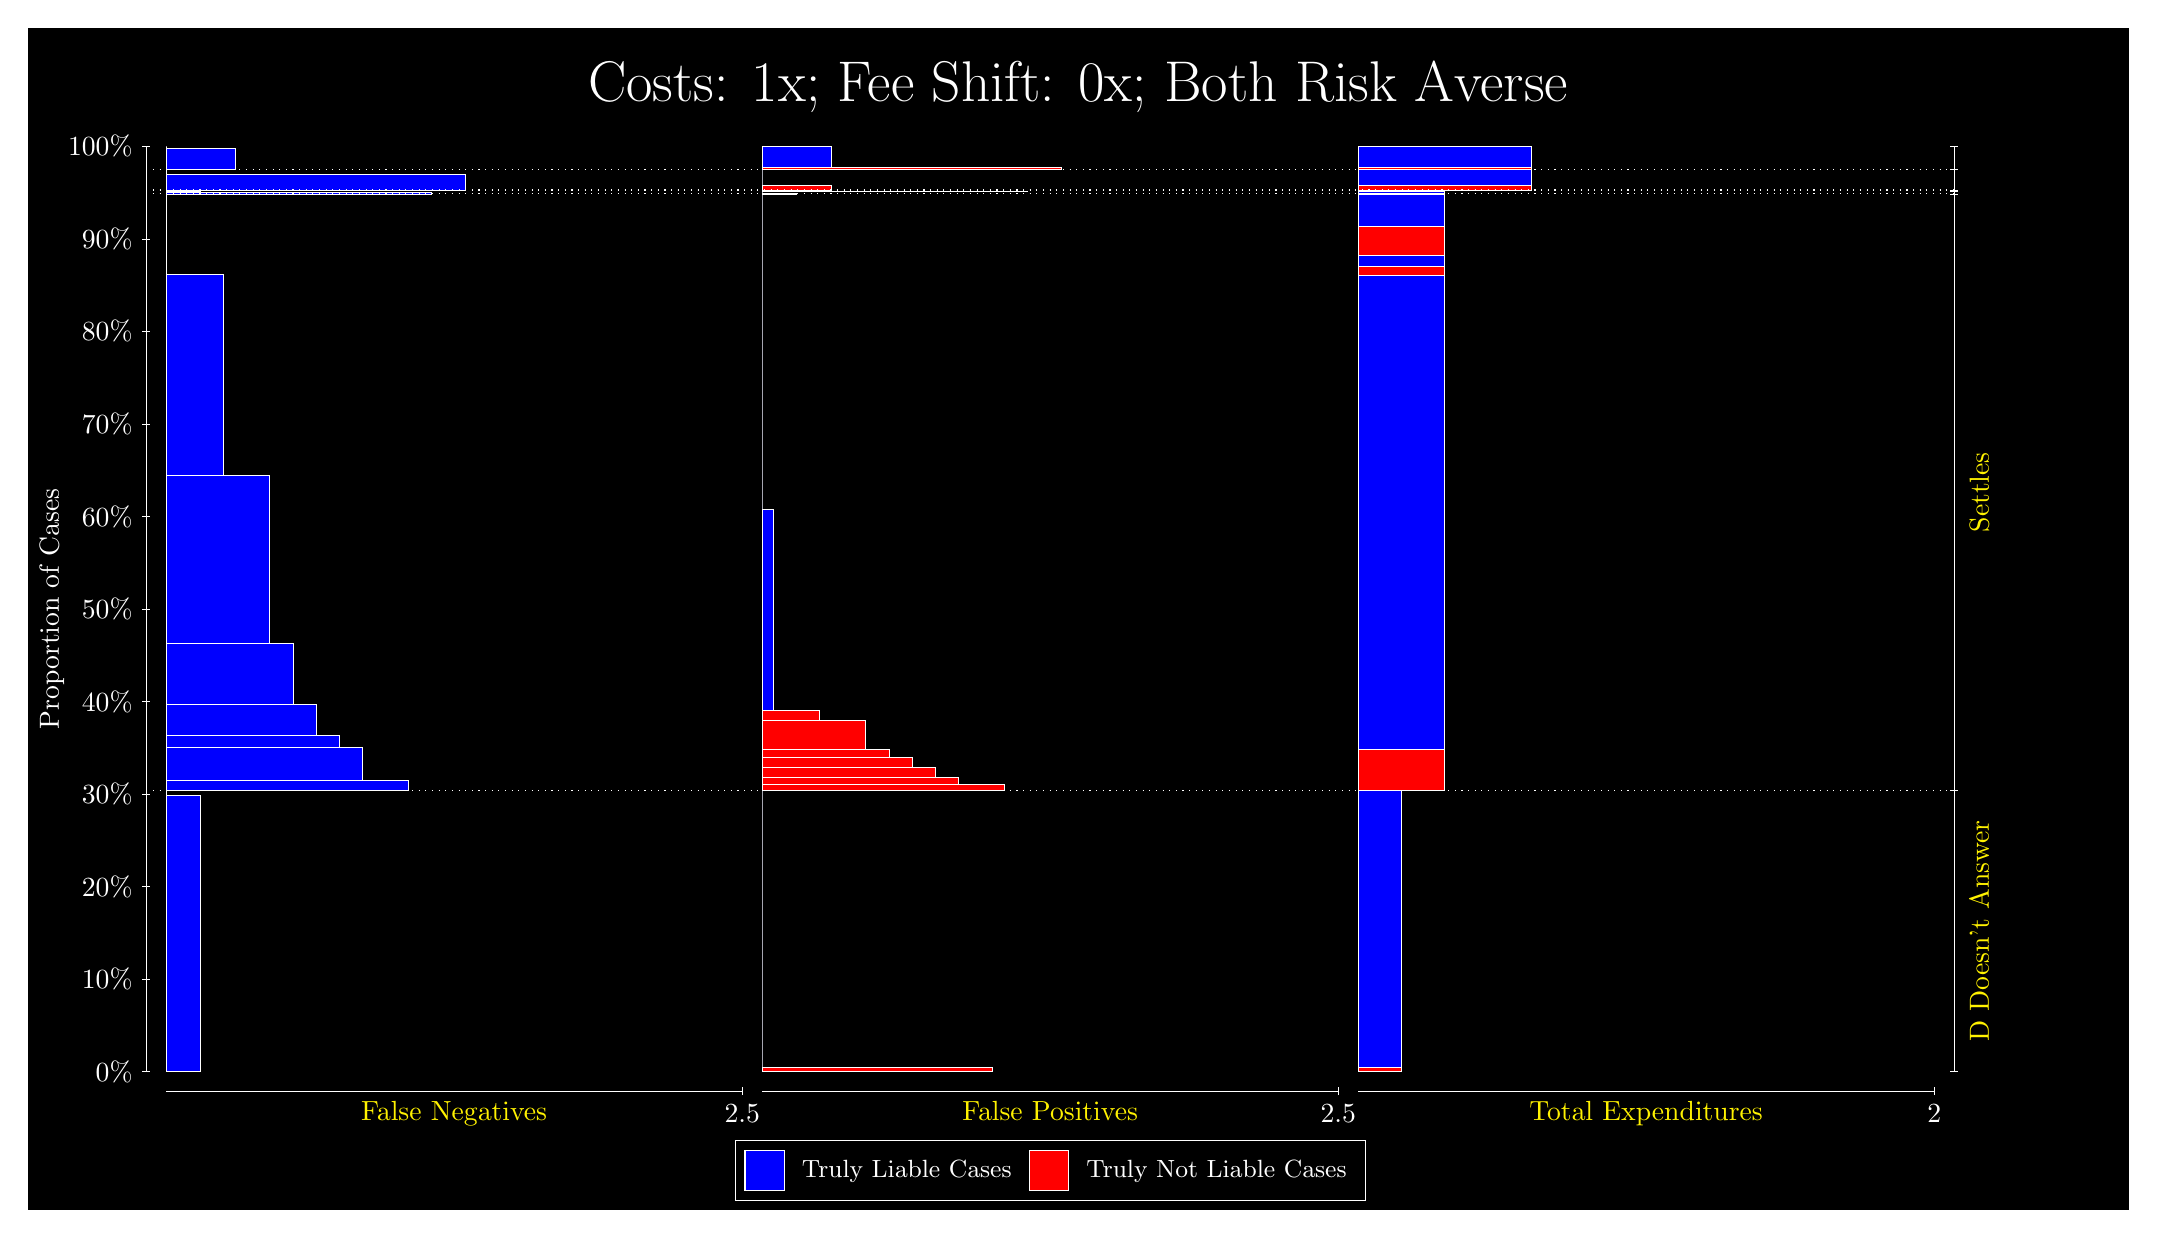
\begin{tikzpicture}
\draw[fill=black] (0,0) rectangle (26.667,15);
\draw[text=white] (0,13.5) rectangle (26.667,15) node[midway] {\huge Costs: 1x; Fee Shift: 0x; Both Risk Averse};
\draw[white, very thin] (1.5,1.75) -- (1.5,13.5);
\node[rotate=90, text=white, anchor=center] at (0.3, 7.625) {Proportion of Cases};
\draw[white, very thin] (1.45,1.75) -- (1.55,1.75);
\node[text=white, anchor=east] at (1.45, 1.75) {0\%};
\draw[white, very thin] (1.45,2.925) -- (1.55,2.925);
\node[text=white, anchor=east] at (1.45, 2.925) {10\%};
\draw[white, very thin] (1.45,4.1) -- (1.55,4.1);
\node[text=white, anchor=east] at (1.45, 4.1) {20\%};
\draw[white, very thin] (1.45,5.275) -- (1.55,5.275);
\node[text=white, anchor=east] at (1.45, 5.275) {30\%};
\draw[white, very thin] (1.45,6.45) -- (1.55,6.45);
\node[text=white, anchor=east] at (1.45, 6.45) {40\%};
\draw[white, very thin] (1.45,7.625) -- (1.55,7.625);
\node[text=white, anchor=east] at (1.45, 7.625) {50\%};
\draw[white, very thin] (1.45,8.8) -- (1.55,8.8);
\node[text=white, anchor=east] at (1.45, 8.8) {60\%};
\draw[white, very thin] (1.45,9.975) -- (1.55,9.975);
\node[text=white, anchor=east] at (1.45, 9.975) {70\%};
\draw[white, very thin] (1.45,11.15) -- (1.55,11.15);
\node[text=white, anchor=east] at (1.45, 11.15) {80\%};
\draw[white, very thin] (1.45,12.325) -- (1.55,12.325);
\node[text=white, anchor=east] at (1.45, 12.325) {90\%};
\draw[white, very thin] (1.45,13.5) -- (1.55,13.5);
\node[text=white, anchor=east] at (1.45, 13.5) {100\%};

\draw[white, very thin] (24.457,1.75) -- (24.457,13.5);
\draw[white, very thin] (24.407,1.75) -- (24.507,1.75);
\node[anchor=west] at (24.407, 1.75) {};
\draw[white, very thin] (24.407,5.318) -- (24.507,5.318);
\node[anchor=west] at (24.407, 5.318) {};
\draw[white, very thin] (24.407,12.896) -- (24.507,12.896);
\node[anchor=west] at (24.407, 12.896) {};
\draw[white, very thin] (24.407,12.934) -- (24.507,12.934);
\node[anchor=west] at (24.407, 12.934) {};
\draw[white, very thin] (24.407,12.947) -- (24.507,12.947);
\node[anchor=west] at (24.407, 12.947) {};
\draw[white, very thin] (24.407,13.207) -- (24.507,13.207);
\node[anchor=west] at (24.407, 13.207) {};
\draw[white, very thin] (24.407,13.5) -- (24.507,13.5);
\node[anchor=west] at (24.407, 13.5) {};

\draw[white, very thin, fill=blue] (1.75,1.75) rectangle (2.1891,5.2581);
\draw[white, very thin, fill=red] (1.75,5.2581) rectangle (1.75,5.318);
\draw[white, very thin, fill=blue] (1.75,5.318) rectangle (4.8239,5.4469);
\draw[white, very thin, fill=blue] (1.75,5.4469) rectangle (4.2384,5.8617);
\draw[white, very thin, fill=blue] (1.75,5.8617) rectangle (3.9457,6.0259);
\draw[white, very thin, fill=blue] (1.75,6.0259) rectangle (3.6529,6.4132);
\draw[white, very thin, fill=blue] (1.75,6.4132) rectangle (3.3602,7.194);
\draw[white, very thin, fill=blue] (1.75,7.194) rectangle (3.0674,9.3221);
\draw[white, very thin, fill=blue] (1.75,9.3221) rectangle (2.4819,11.879);
\draw[white, very thin, fill=red] (1.75,11.879) rectangle (1.75,12.896);
\draw[white, very thin, fill=blue] (1.75,12.896) rectangle (5.1167,12.922);
\draw[white, very thin, fill=red] (1.75,12.922) rectangle (1.75,12.934);
\draw[white, very thin, fill=blue] (1.75,12.934) rectangle (2.1891,12.946);
\draw[white, very thin, fill=red] (1.75,12.946) rectangle (1.75,12.947);
\draw[white, very thin, fill=blue] (1.75,12.947) rectangle (5.5558,13.143);
\draw[white, very thin, fill=red] (1.75,13.143) rectangle (1.75,13.207);
\draw[white, very thin, fill=blue] (1.75,13.207) rectangle (2.6283,13.478);
\draw[white, very thin, fill=red] (1.75,13.478) rectangle (1.75,13.5);
\draw[white, very thin, fill=red] (9.3189,1.75) rectangle (12.246,1.8098);
\draw[white, very thin, fill=blue] (9.3189,1.8098) rectangle (9.3189,5.318);
\draw[white, very thin, fill=red] (9.3189,5.318) rectangle (12.393,5.3944);
\draw[white, very thin, fill=red] (9.3189,5.3944) rectangle (11.807,5.4858);
\draw[white, very thin, fill=red] (9.3189,5.4858) rectangle (11.515,5.6137);
\draw[white, very thin, fill=red] (9.3189,5.6137) rectangle (11.222,5.7417);
\draw[white, very thin, fill=red] (9.3189,5.7417) rectangle (10.929,5.8435);
\draw[white, very thin, fill=red] (9.3189,5.8435) rectangle (10.636,6.2149);
\draw[white, very thin, fill=red] (9.3189,6.2149) rectangle (10.051,6.3352);
\draw[white, very thin, fill=blue] (9.3189,6.3352) rectangle (9.4652,8.8923);
\draw[white, very thin, fill=blue] (9.3189,8.8923) rectangle (9.3189,12.896);
\draw[white, very thin, fill=red] (9.3189,12.896) rectangle (9.758,12.908);
\draw[white, very thin, fill=blue] (9.3189,12.908) rectangle (9.3189,12.934);
\draw[white, very thin, fill=red] (9.3189,12.934) rectangle (12.686,12.935);
\draw[white, very thin, fill=blue] (9.3189,12.935) rectangle (9.758,12.947);
\draw[white, very thin, fill=red] (9.3189,12.947) rectangle (10.197,13.01);
\draw[white, very thin, fill=blue] (9.3189,13.01) rectangle (9.3189,13.207);
\draw[white, very thin, fill=red] (9.3189,13.207) rectangle (13.125,13.228);
\draw[white, very thin, fill=blue] (9.3189,13.228) rectangle (10.197,13.5);
\draw[white, very thin, fill=red] (16.888,1.75) rectangle (17.437,1.8098);
\draw[white, very thin, fill=blue] (16.888,1.8098) rectangle (17.437,5.318);
\draw[white, very thin, fill=red] (16.888,5.318) rectangle (17.986,5.8435);
\draw[white, very thin, fill=blue] (16.888,5.8435) rectangle (17.986,11.861);
\draw[white, very thin, fill=red] (16.888,11.861) rectangle (17.986,11.981);
\draw[white, very thin, fill=blue] (16.888,11.981) rectangle (17.986,12.11);
\draw[white, very thin, fill=red] (16.888,12.11) rectangle (17.986,12.482);
\draw[white, very thin, fill=blue] (16.888,12.482) rectangle (17.986,12.896);
\draw[white, very thin, fill=red] (16.888,12.896) rectangle (17.986,12.908);
\draw[white, very thin, fill=blue] (16.888,12.908) rectangle (17.986,12.934);
\draw[white, very thin, fill=red] (16.888,12.934) rectangle (17.986,12.935);
\draw[white, very thin, fill=blue] (16.888,12.935) rectangle (17.986,12.947);
\draw[white, very thin, fill=red] (16.888,12.947) rectangle (19.083,13.01);
\draw[white, very thin, fill=blue] (16.888,13.01) rectangle (19.083,13.207);
\draw[white, very thin, fill=red] (16.888,13.207) rectangle (19.083,13.228);
\draw[white, very thin, fill=blue] (16.888,13.228) rectangle (19.083,13.5);
\draw[white, dotted] (1.5,5.318) -- (24.457,5.318);
\draw[white, dotted] (1.5,12.896) -- (24.457,12.896);
\draw[white, dotted] (1.5,12.934) -- (24.457,12.934);
\draw[white, dotted] (1.5,12.947) -- (24.457,12.947);
\draw[white, dotted] (1.5,13.207) -- (24.457,13.207);
\draw[white, very thin] (1.75,1.5) -- (9.0689,1.5);
\node[text=yellow, anchor=north] at (5.4094, 1.5) {False Negatives};
\draw[white, very thin] (9.0689,1.45) -- (9.0689,1.55);
\node[text=white, anchor=north] at (9.0689, 1.45) {2.5};

\draw[white, very thin] (9.3189,1.5) -- (16.638,1.5);
\node[text=yellow, anchor=north] at (12.978, 1.5) {False Positives};
\draw[white, very thin] (16.638,1.45) -- (16.638,1.55);
\node[text=white, anchor=north] at (16.638, 1.45) {2.5};

\draw[white, very thin] (16.888,1.5) -- (24.207,1.5);
\node[text=yellow, anchor=north] at (20.547, 1.5) {Total Expenditures};
\draw[white, very thin] (24.207,1.45) -- (24.207,1.55);
\node[text=white, anchor=north] at (24.207, 1.45) {2};

\node[text=yellow, centered, rotate=90] at (24.777, 3.534) {D Doesn't Answer};
\node[text=yellow, centered, rotate=90] at (24.777, 9.1072) {Settles};





\draw (12.978300999999998,1.5) node[draw=none] (baseCoordinate) {};
\begin{scope}[align=center]
        \matrix[scale=0.5, draw=white, below=0.5cm of baseCoordinate, nodes={draw}, column sep=0.1cm]{
            \node[rectangle, draw, minimum width=0.5cm, minimum height=0.5cm, fill=blue] {}; &
            \node[draw=none, font=\small, text=white] (B) {Truly Liable Cases}; &
            \node[rectangle, draw, minimum width=0.5cm, minimum height=0.5cm, fill=red] {}; &
            \node[draw=none, font=\small, text=white] (B) {Truly Not Liable Cases}; \\
            };
\end{scope}

\end{tikzpicture}
\end{document}